\documentclass{beamer}
\usetheme{Madrid}
\usepackage[utf8]{inputenc}
\usepackage{amsmath,amssymb}
\usepackage{graphicx}

\title{Vortex Flow: Numerical Simulation of the Taylor--Green Vortex}
\author{Masud}
\date{\today}

\begin{document}

% Title Slide
\begin{frame}
\titlepage
\end{frame}

% Outline
\begin{frame}{Outline}
\tableofcontents
\end{frame}

% Introduction
\section{Introduction}
\begin{frame}{Vortex Flow}
Vortex flows represent rotational motion of fluid elements, fundamental to turbulence, mixing, and aerodynamics.

The \textbf{Taylor--Green vortex} is a canonical test problem for CFD:
\[
\begin{aligned}
u(x,y,0) &= U_0 \sin(kx) \cos(ky), \\
v(x,y,0) &= -U_0 \cos(kx) \sin(ky), \\
p(x,y,0) &= \frac{\rho U_0^2}{4} \big[\cos(2kx) + \cos(2ky)\big].
\end{aligned}
\]

\begin{itemize}
    \item Incompressible, viscous, two-dimensional flow
    \item Initially periodic velocity field
    \item Decays over time due to viscosity
\end{itemize}
\end{frame}

% Governing Equations
\section{Governing Equations}
\begin{frame}{Navier--Stokes Equations}
\[
\begin{aligned}
\frac{\partial \mathbf{u}}{\partial t} + (\mathbf{u} \cdot \nabla)\mathbf{u} &= -\nabla p + \nu \nabla^2 \mathbf{u}, \\
\nabla \cdot \mathbf{u} &= 0.
\end{aligned}
\]

\begin{itemize}
    \item Viscosity $\nu$ controls vortex decay rate
    \item Periodic boundary conditions in both directions
\end{itemize}
\end{frame}

% Analytical Solution
\section{Analytical Solution}
\begin{frame}{Analytical Solution (Decay of Vortex)}
The velocity field decays exponentially due to viscosity:
\[
\begin{aligned}
u(x,y,t) &= U_0 \sin(kx)\cos(ky)\, e^{-2\nu k^2 t}, \\
v(x,y,t) &= -U_0 \cos(kx)\sin(ky)\, e^{-2\nu k^2 t}.
\end{aligned}
\]

\begin{itemize}
    \item The structure remains identical over time
    \item Amplitude decreases with $e^{-2\nu k^2 t}$
\end{itemize}
\end{frame}

% Numerical Method
\section{Numerical Method}
\begin{frame}{Discretization and Simulation}
\begin{itemize}
    \item Spatial discretization: central differences for derivatives
    \item Time integration: explicit schemes (RK2, RK4)
    \item Pressure projection step enforces $\nabla \cdot \mathbf{u} = 0$
    \item Periodic boundary conditions applied in both $x$ and $y$
\end{itemize}
\end{frame}

% Example
\section{Example}
\begin{frame}{Velocity Field}
\begin{figure}[h]
\centering
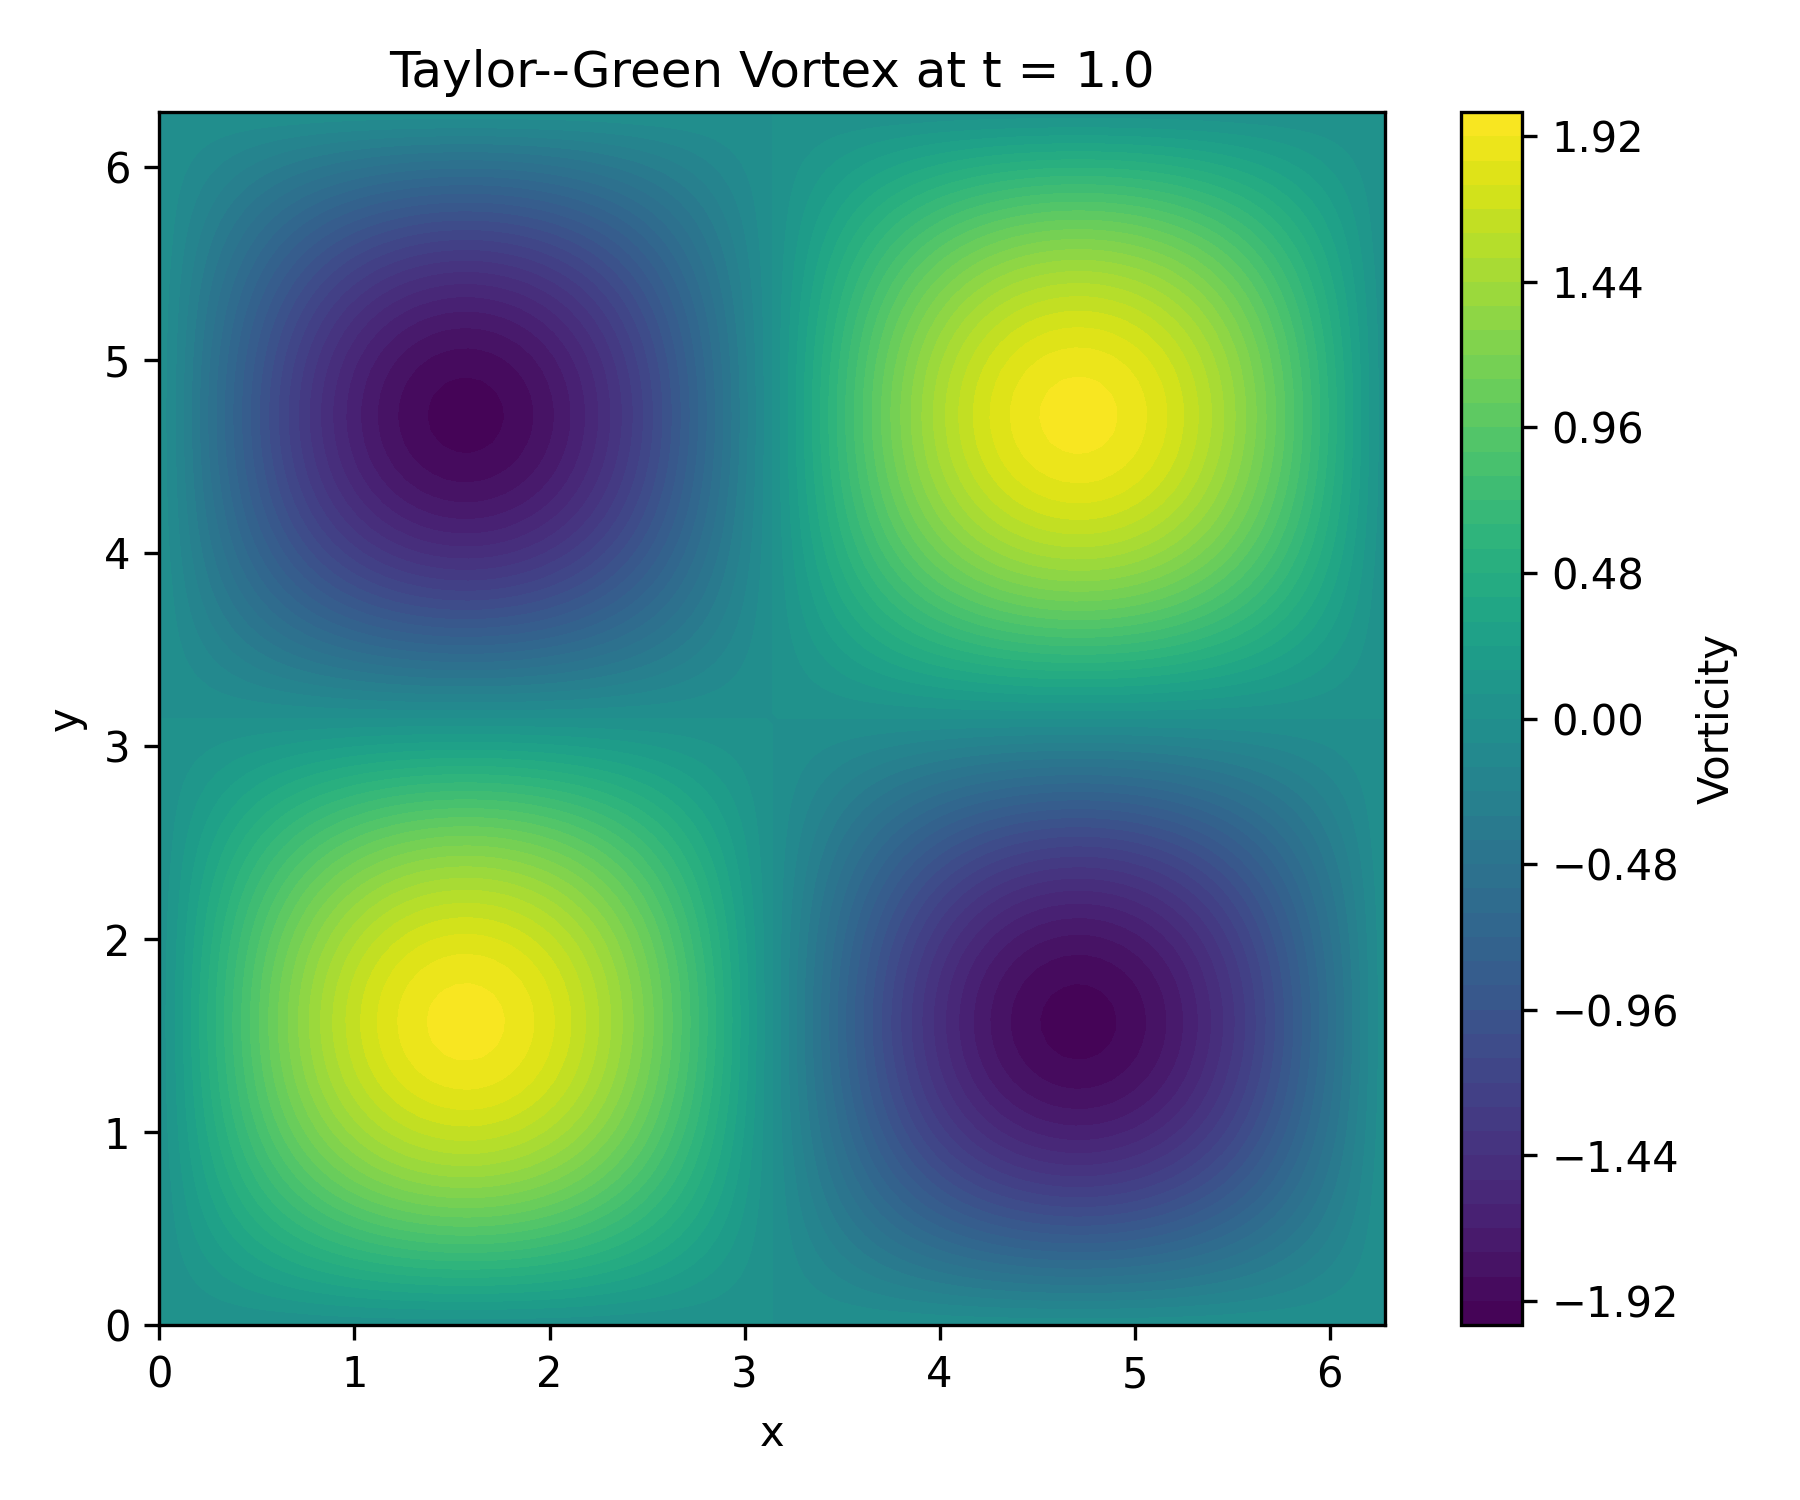
\includegraphics[width=0.8\linewidth]{vortex_plot.png} % replace with your figure
\caption{Taylor--Green vortex: vorticity field at time $t = 1.0$}
\end{figure}
\end{frame}

% Discussion
\section{Discussion}
\begin{frame}{Observations}
\begin{itemize}
    \item Energy decays exponentially with viscosity
    \item Flow remains symmetric and periodic
    \item Excellent benchmark for assessing numerical dissipation and accuracy
\end{itemize}
\end{frame}

% Conclusion
\section{Conclusion}
\begin{frame}{Conclusion}
\begin{itemize}
    \item The Taylor--Green vortex demonstrates fundamental vortex dynamics
    \item Used extensively for CFD solver validation
    \item Provides analytical reference for numerical error analysis
\end{itemize}
\end{frame}

\end{document}